\documentclass[a4paper,12pt]{article}

% Pacchetti fondamentali
\usepackage[utf8]{inputenc}   % Codifica caratteri
\usepackage[italian]{babel}    % Lingua italiana
\usepackage{amsmath}           % Formule matematiche avanzate
\usepackage{graphicx}          % Inserimento immagini
\usepackage{geometry}          % Gestione margini
 \geometry{margin=2.5cm}
\usepackage{booktabs}          % Tabelle professionali
\usepackage{physics}
\usepackage{float}
\usepackage{caption}
\usepackage{textcomp}
\usepackage{amssymb}
\usepackage{parskip}

\title{Misura della costante elastica di una molla elicoidale}
\author{Eddi Bressan, Davide Conforte}
\date{\today}

\begin{document}

\maketitle
\tableofcontents
\newpage

\section{Obiettivo dell'esperienza}
Lo scopo dell'esperienza è lo studio della deformazione di una molla elicoidale tramite due metodi: statico e dinamico.

\section{Cenni teorici}

\subsection{Deformazione elastica}
Una deformazione è detta \textbf{elastica} se il corpo torna allo stato originario quando
vengono meno le forze che l'hanno causata.

Questo comportamento si mantiene se le forze applicate sono inferiori
ad un limite dipendente da vari fattori: materiale, temperatura, tipo di deformazione considerata, etc.

Nelle deformazioni elastiche si osserva una relazione di proporzionalità tra sollecitazione e deformazione:
$$
\Delta L \propto F
$$
\noindent
Questo comportamento è noto come \textbf{legge di Hooke}.

La legge di Hooke è valida per la maggior parte dei minerali, per il vetro,
per i materiali ceramici e per i metalli. Per i materiali duttili invece è vera per carichi modesti.

Quando all'estremità libera di una molla è applicata una forza,
la molla esercita una forza di richiamo proporzionale allo spostamento di tale 
estremo rispetto alla posizione di equilibrio.

Il modulo della forza di richiamo è proporzionale alla deformazione (legge di Hooke):
$$
\vec{F} = -k \vec{x}
$$
Dove $\vec{x}$ è la deformazione della molla rispetto la sua lunghezza a riposo $\vec{x} = (l - l_{0})\hat{x}$
con $l_0$ la lunghezza della molla a riposo.

La costante di proporzionalità $k$ è detta \textbf{costante elastica} della molla e 
dipende dal materiale di cui è costituita, dal diametro del filo e dal numero di spire della molla.


\subsection{Metodo statico}
La costante elastica di una molla può essere determinata sperimentalmente misurando
le elongazioni $\Delta l$ al variare delle forze applicate.

Se all'estremità inferiore di una molla sospesa verticalmente è appesa una massa m,
la forza applicata coincide con la forza peso della massa e la legge di Hooke si riscrive
nel seguente modo:
$$
mg = k {\Delta l} = k (l-l_0)
$$
Usando diverse masse e misurando i rispettivi $\Delta l$ si ottengono diverse misure di k:
$$
k_i = \frac{m_i g}{\Delta l_i}
$$
Nella configurazione reale, alla molla è appeso un piattello (di massa $m_p$).
Inoltre, possedendo una massa propria, la molla è soggetta alla forza di gravità e subisce pertanto un allungamento iniziale $l_s$ anche a piattello scarico.

Misurando la differenza tra l'allungamento a piatto scarico:
$$
(m_p + m_{eff.statica})g = k(l_s - l_0)
$$
e l'allungamento in seguito all'aggiunta di una massa $m_i$:
$$
(m_i + m_p + m_{eff.statica})g = k(l_i - l_0)
$$
e sottraendo membro a membro le due equazioni si ottiene:
$$
m_i g = k_i (l_i - l_s)
$$
Da cui il valore della costante elastica della molla:
$$
k_i = \frac{m_i g}{(l_i - l_s)}
$$
Le incertezze sono interamente dovute alla sensibilità strumentale, pertanto si può scrivere:
$$
\frac{\Delta k_i}{k_i} = \frac{\Delta m_i}{m_i}+2\frac{\Delta l}{(l_i - l_s)}
$$

\subsection{Metodo dinamico}
Partendo dalla legge di Hooke:
$$
mg = k \Delta l = k(l_{eq} - l_0)
$$
Se applicando una forza, si sposta la massa dalla sua posizione di equilibrio e la si rilascia,
il sistema inizierà ad oscillare attorno alla posizione di equilibrio $l_{0}$ con equazione:
$$
m\ddot{x} + kx = mg
$$
La soluzione di questa equazione differenziale sarà data da una soluzione dell'equazione
omogenea:
$$
m\ddot{x} + kx = 0 \quad \text{o} \quad \ddot{x} + \frac{k}{m}x = 0
$$
Sommata ad una soluzione particolare dell'equazione non omogenea.
Le condizioni iniziali sono:
$$
\begin{cases}
    \dot{x}(t=0)=0 \\
    x(t=0)=x_0
\end{cases}
$$
La soluzione dell'equazione differenziale omogenea è del tipo $x(t) = A \sin(\omega t+\phi)$
mentre una soluzione particolare dell'equazione non omogenea è la soluzione costante:
$$
x = \frac{mg}{k} = l_{eq} - l_0
$$
La soluzione completa è quindi:
$$
x(t) = A \sin(\omega t+\phi) + l_{eq} - l_0
$$
Con:
$$
\begin{cases}
    \dot{x}(t=0)=0 \\
    x(t=0)=x_0
\end{cases}
$$
Si ha quindi:
$$
\begin{cases}
    \dot{x} = A \omega \cos(\omega t + \phi) = 0 \\
    \ddot{x} = -A \omega^2 \sin(\omega t + \phi)
\end{cases}
$$
Da cui si ricava:
$$
-A \omega^2 \sin(\omega t + \phi) + \frac{k}{m} A \sin(\omega t + \phi) + \frac{k}{m}[l_{eq} - l_0] = g
$$
È perciò necessario che valga:
$$
\omega = \sqrt{\frac{k}{m}}
$$
Ovvero la pulsazione non cambia a causa della forza di gravità.

La condizione iniziale $\dot{x}(t=0)=0$ fornisce:
$$
\cos(\phi) = 0 \quad \text{o} \quad \phi = \frac{\pi}{2} 
$$
Mentre, applicando la condizione $x(t=0)=x_0$, si ottiene:
$$
x_0 = A + l_{eq} - l_0
$$
Da cui:
$$
A = x_0 - (l_{eq} - l_0)
$$
Per una soluzione completa data da:
$$
x(t) = [x_0 - (l_{eq} - l_0)]\sin(\sqrt{\frac{k}{m}}t+\frac{\pi}{2}) + (l_{eq} - l_0) 
$$
Il fatto che $\omega = \sqrt{\frac{k}{m}}$ permette di calcolare la costante elastica della molla dalla
misura del periodo di oscillazione:
$$
T = \frac{2\pi}{\omega} = 2\pi \sqrt{\frac{m}{k}}
$$
In questo caso, è necessario considerare la massa totale sospesa, inclusa quella del supporto.

\subsection{Massa efficace dinamica}
Nella misura tramite metodo dinamico non si può trascurare la massa della molla in relazione alla stima del
periodo di oscillazione.
Si dovrà valutare il contributo di $m_m$ anche in questo caso come $m_{eff.dinamica}$

Si calcoli la variazione dell'energia cinetica $dK$ della molla a causa della stessa massa $dm$ di un 
elemento di lunghezza $dx$ che si muove con una velocità istantanea $v$ durante il moto armonico della molla:
$$
dK = \frac{1}{2}dmv^2
$$
Poiché vale $dm = m_m \frac{dx}{l}$, mentre la velocità alla distanza x sarà legata alla velocità all'estremo
$l$ della molla V da:
$$
v = \frac{x}{l}V
$$
Si può quindi scrivere:
$$
dK = \frac{1}{2}(\frac{x}{l}V)^2 \frac{m_m}{l}dx
$$
L'energia cinetica totale della molla in oscillazione si ottiene integrando da 0 alla lunghezza della molla $l$:
$$
K = \frac{1}{2}(\frac{V}{l})^2 \frac{m_m}{l} \int_{0}^{l} x^2 dx
$$
Ovvero:
$$
K = \frac{1}{2}(\frac{V}{l})^2 \frac{m_m}{l} \frac{l^3}{3} = \frac{1}{2}V^2 \frac{m_m}{3}
$$
Sommando anche la massa appesa alla molla (anch'essa in movimento con velocità $V$) si ottiene un'energia
cinetica totale:
$$
K = \frac{1}{2}V^2 (m+\frac{m_m}{3})
$$
Pertanto, la massa efficace della molla da sommare alla massa appesa è, nel caso dinamico,
pari a:

$$
m_{eff.dinamica} = \frac{m_m}{3}
$$
\subsection{I due modelli utilizzati}
Si può evitare di utilizzare il modello della massa efficace in questo modo:
\begin{equation*}
    T_i^2 = 4\pi^2 \frac{\frac{m_m}{3} + m_p + m_i}{k} \quad \text{e} \quad T_{0,i}^2 = 4\pi^2 \frac{\frac{m_m}{3} + m_p}{k}
\end{equation*}
dove $T_{0,i}$ è il periodo di oscillazione a piatto scarico.
\begin{equation*}
    T_i^2 - T_{0,i}^2 = 4\pi^2 \frac{m_i}{k}
\end{equation*}
Seguendo questo approccio risulta necessario prendere un set di misure a piatto scarico per ogni massa $m_i$ in modo che i valori calcolati siano indipendenti.



\subsection{Metodo dinamico con attriti}
Nel caso in cui non si possano trascurare gli attriti, è necessario inserire un termine proporzionale al
$dx/dt$ che dipenderà dalla viscosità del mezzo (e da eventuali attriti meccanici nella molla stessa).
Si consideri per semplicità l'equazione omogenea (la cui soluzione particolare è già stata discussa):
$$
m\ddot{x} + C\dot{x} + kx = 0
$$
Ovvero:
$$
\ddot{x} + \frac{C}{m} \dot{x} + \frac{k}{m} x = 0
$$
Con condizioni iniziali:
$$
x(t=0) = x_0 \quad \text{e} \quad \dot{x}(t=0) = 0
$$
E con, per comodità:
$$
2\gamma = \frac{C}{m} \quad \text{e} \quad \omega_0 = \sqrt{\frac{k}{m}}
$$
Ovvero:
$$
\ddot{x} + 2\gamma \dot{x} + \omega_0^2 x = 0
$$
Che è un'equazione differenziale lineare di secondo ordine a coefficienti costanti.

Dalla teoria delle equazioni differenziali si ricava la legge oraria del moto:
$$
x(t) = A e^{\gamma t} \cos(\sqrt{\omega_0^2 - \gamma^2 t} + \phi) \quad \text{per} \quad \gamma < \omega_0
$$
Si ottiene quindi un moto oscillatorio smorzato, con A e $\phi$ che dipendono dalle condizioni iniziali.
Si nota che la pulsazione misurata è influenzata dall'attrito:
$$
\omega_0 \to \omega_0 - \frac{C}{2m}
$$

\newpage
\section{Apparato sperimentale}
\textbf{Strumenti di misura}
\begin{table}[htbp]
    \centering
    \begin{tabular}{lr} % l = left (allineato a sinistra), c = center (centrato)
        \toprule
        \textbf{Strumento} & \textbf{Risoluzione} \\
        \midrule
        Metro a nastro      & $1$ mm               \\
        Cronometro digitale & $0.01$ s             \\
        Bilancia analitica    & $0.01$ g              \\
        \bottomrule
    \end{tabular}
\end{table}\\
\textbf{Componenti del sistema fisico}
\begin{table}[htbp]
    \centering
    \footnotesize
    \vspace{8pt} % Spazio aggiuntivo tra didascalia e tabella
    \begin{tabular}{lll}
        \toprule
        \textbf{Elemento} & \textbf{Proprietà} & \textbf{Valore Nominale} \\
        \midrule
        Massa oscillante (Piattello) & Massa ($M_p$)     & 20.10 g                \\
        Massa appesa                 & Massa ($M_i$)  & variabile (4.97 - 49.99)g \\
        \addlinespace
        Molla      & Massa ($M_m$)     &  29.96 g                  \\
                                 & Lunghezza ($l_i$) & variabile (19.9 - 65.3) cm           \\
        \addlinespace
        Stativo                  & Supporto rigido   & ---                    \\
        \bottomrule
    \end{tabular}
\end{table}

\section{Procedura sperimentale}
\subsection{Misure preliminari}
\begin{itemize}
    \item Misura della massa della molla $M_m$, del piattello $M_p$ e delle masse $M_i$.
    \item Misura della lunghezza della molla a riposo $l_0$.
\end{itemize}

\subsection{Set-up dell'apparato}     
\subsubsection{Misura tramite metodo statico}
\begin{itemize}
    \item \textbf{Misura della lunghezza a riposo ($l_0$):} La molla è stata inizialmente vincolata al supporto verticale (stativo) lasciandola pendere liberamente in assenza di carichi applicati. Tramite il metro, è stata rilevata la quota corrispondente all'estremità inferiore della molla, registrando tale valore come lunghezza intrinseca a riposo $l_0$.
    
    \item \textbf{Misura a piattello scarico ($l_s$):} Si è proceduto ad agganciare il piattello porta-masse vuoto all'estremità inferiore del sistema. Una volta raggiunto l'equilibrio statico, è stata misurata la nuova lunghezza della molla $l_s$
    
    \item \textbf{Applicazione incrementale dei carichi:} Sull'apposito piattello sono state posizionate, in successione e una alla volta, le masse campionate a disposizione.
    
    \item \textbf{Rilevazione delle lunghezze in equilibrio:} Raggiunta la condizione stazionaria di equilibrio meccanico (in cui la forza elastica della molla bilancia esattamente la forza peso totale), si è effettuata la lettura della lunghezza finale.
    
    \item \textbf{Ripetibilità e campionamento dei dati:} L'intera procedura di carico è stata reiterata per un totale di 5 volte con masse differenti.
\end{itemize}
\subsubsection{Misura tramite metodo dinamico}
\begin{itemize}
    \item \textbf{Selezione e configurazione delle masse:} Sono state selezionate 5 differenti masse per studiare la dipendenza del periodo di oscillazione $T$ in funzione della massa totale sospesa.
    
    \item \textbf{Misura del tempo cumulativo:} Per ciascuna massa, dopo aver impresso un piccolo spostamento verticale rispetto alla posizione di equilibrio, il sistema è stato lasciato oscillare liberamente. Al fine di minimizzare l'incertezza associata al tempo di reazione dell'operatore nell'attivazione e nell'arresto del cronometro, non è stato misurato un singolo periodo, bensì un intervallo comprendente 5 oscillazioni complete.
    
    \item \textbf{Reiterazione e struttura dei set di dati:} Per ognuna delle 5 configurazioni a masse diverse la misura di $\tau = 5T$ è stata ripetuta 10 volte.
    
    \item \textbf{Misure indipendenti a piattello scarico:} In corrispondenza di ciascuna delle sessioni di misura relative alle 5 masse, è stato acquisito un set indipendente di misure considerando il solo piattello scarico. Questa operazione di calibrazione locale è cruciale per la successiva elaborazione dati.
\end{itemize}

\section{Risultati delle Misure}

In questa sezione vengono riportati esclusivamente i dati grezzi raccolti direttamente tramite le misurazioni in laboratorio, prima di procedere a qualsiasi elaborazione statistica o analisi fisica. I dati si riferiscono all'unica molla utilizzata durante l'esperienza.

\subsection{Misure Statiche}
Per la caratterizzazione statica della molla, sono state rilevate le lunghezze corrispondenti ai diversi carichi applicati. Le misure di riferimento iniziale sono:
\begin{itemize}
    \item \textbf{Lunghezza della molla a riposo ($l_0$):} 19.9 cm
    \item \textbf{Lunghezza della molla a piattello scarico ($l_s$):} 32.4 cm
\end{itemize}

Nella Tabella~\ref{tab:misure_statiche} sono elencati i valori delle masse nominali inserite e le corrispondenti lunghezze totali della molla lette sul regolo millimetrato.

\begin{table}[h!]
\centering
\begin{tabular}{cc}
\hline
\textbf{Massa applicata $m_i$ (g)} & \textbf{Lunghezza misurata $l_i$ (cm)} \\ \hline
4.97 & 35.7 \\
10.30 & 38.9 \\
20.00 & 45.6 \\
30.03 & 52.3 \\
49.99 & 65.3 \\ \hline
\end{tabular}
\caption{Dati grezzi delle misure statiche: masse applicate e lunghezze complessive della molla.}
\label{tab:misure_statiche}
\end{table}

\subsection{Misure Dinamiche ed Istogrammi delle Distribuzioni}
Per la caratterizzazione dinamica sono state impiegate 5 configurazioni di massa differenti. Ciascuna sessione prevede l'acquisizione del tempo totale impiegato dal sistema per compiere 5 oscillazioni complete ($\tau$). 

Per ogni massa, la misura è stata ripetuta per 10 volte consecutive sia nella condizione di piattello scarico (riferimento indipendente), sia nella condizione di piattello carico. Di seguito vengono riportate le tabelle dei tempi grezzi affiancate dai rispettivi istogrammi per la verifica della distribuzione normale dei dati.

% ==========================================
% MASSA 1
% ==========================================
\subsubsection*{Configurazione Massa $m_1 = 4,97$ g}
\noindent
\begin{minipage}[c]{0.45\textwidth}
\centering
\small
\begin{tabular}{ccc}
\hline
\textbf{Ripetizione} & \textbf{Scarico (s)} & \textbf{Carico (s)} \\ \hline
1  & 4.41 & 4.86 \\
2  & 4.43 & 5.00 \\
3  & 4.44 & 4.96 \\
4  & 4.49 & 4.84 \\
5  & 4.41 & 4.90 \\
6  & 4.56 & 5.03 \\
7  & 4.34 & 4.91 \\
8  & 4.55 & 5.06 \\
9  & 4.43 & 4.94 \\
10 & 4.46 & 4.83 \\ \hline
\end{tabular}
\captionof{table}{Tempi grezzi (5 oscillazioni) per la Massa 1.}
\label{tab:dinamica_massa1}
\end{minipage}
\hfill
\begin{minipage}[r]{0.70\textwidth}
    \centering
    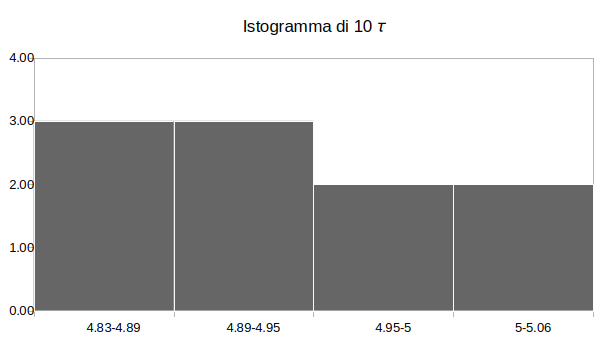
\includegraphics[width=0.8\textwidth]{Immagini/istogramma_dinamico_1.png}
    \captionof{figure}{Istogramma delle 10 misure.}
\end{minipage}

\vspace{0.8cm} % Spazio verticale prima della massa successiva

% ==========================================
% MASSA 2
% ==========================================
\subsubsection*{Configurazione Massa $m_2 = 10.30$ g}
\noindent
\begin{minipage}[c]{0.45\textwidth}
\centering
\small
\begin{tabular}{ccc}
\hline
\textbf{Ripetizione} & \textbf{Scarico (s)} & \textbf{Carico (s)} \\ \hline
1  & 4.42 & 5.16 \\
2  & 4.37 & 5.18 \\
3  & 4.41 & 5.35 \\
4  & 4.40 & 5.26 \\
5  & 4.46 & 5.13 \\
6  & 4.40 & 5.16 \\
7  & 4.46 & 5.20 \\
8  & 4.49 & 5.12 \\
9  & 4.41 & 5.06 \\
10 & 4.43 & 5.15 \\ \hline
\end{tabular}
\captionof{table}{Tempi grezzi (5 oscillazioni) per la Massa 2.}
\label{tab:dinamica_massa2}
\end{minipage}
\hfill
\begin{minipage}[r]{0.70\textwidth}
    \centering
    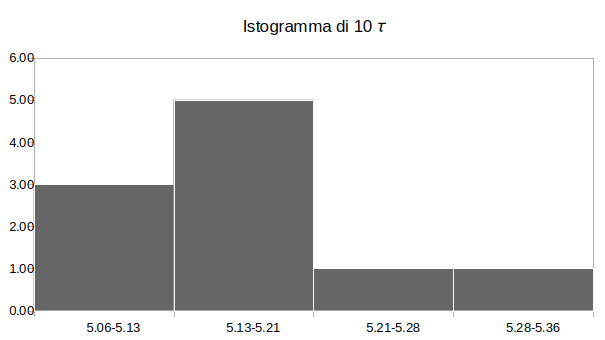
\includegraphics[width=0.8\textwidth]{Immagini/istogramma_dinamico_2.png}
    \captionof{figure}{Istogramma delle 10 misure.}
\end{minipage}


\vspace{0.8cm}

% ==========================================
% MASSA 3
% ==========================================
\subsubsection*{Configurazione Massa $m_3 = 20.00$ g}
\noindent
\begin{minipage}[c]{0.45\textwidth}
\centering
\small
\begin{tabular}{ccc}
\hline
\textbf{Ripetizione} & \textbf{Scarico (s)} & \textbf{Carico (s)} \\ \hline
1  & 4.50 & 5.76 \\
2  & 4.46 & 5.78 \\
3  & 4.45 & 6.00 \\
4  & 4.35 & 5.86 \\
5  & 4.46 & 5.96 \\
6  & 4.50 & 5.86 \\
7  & 4.43 & 5.93 \\
8  & 4.41 & 5.80 \\
9  & 4.41 & 5.72 \\
10 & 4.40 & 5.87 \\ \hline
\end{tabular}
\captionof{table}{Tempi grezzi (5 oscillazioni) per la Massa 3.}
\label{tab:dinamica_massa3}
\end{minipage}
\hfill
\begin{minipage}[r]{0.70\textwidth}
    \centering
    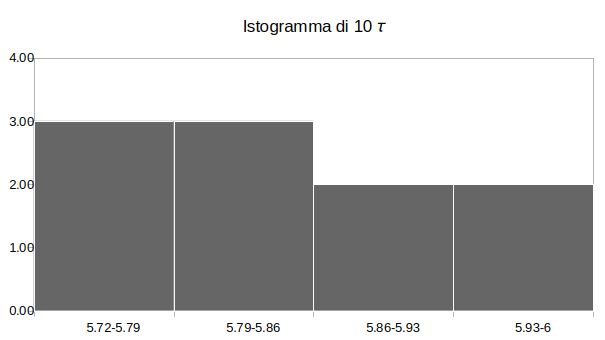
\includegraphics[width=0.8\textwidth]{Immagini/istogramma_dinamico_3.png}
    \captionof{figure}{Istogramma delle 10 misure.}
\end{minipage}

\vspace{0.8cm}

% ==========================================
% MASSA 4
% ==========================================
\subsubsection*{Configurazione Massa $m_4 = 30.03$ g}
\noindent
\begin{minipage}[c]{0.45\textwidth}
\centering
\small
\begin{tabular}{ccc}
\hline
\textbf{Ripetizione} & \textbf{Scarico (s)} & \textbf{Carico (s)} \\ \hline
1  & 4.40 & 6.40 \\
2  & 4.38 & 6.27 \\
3  & 4.41 & 6.37 \\
4  & 4.46 & 6.35 \\
5  & 4.35 & 6.32 \\
6  & 4.46 & 6.29 \\
7  & 4.43 & 6.41 \\
8  & 4.43 & 6.27 \\
9  & 4.46 & 6.27 \\
10 & 4.40 & 6.41 \\ \hline
\end{tabular}
\captionof{table}{Tempi grezzi (5 oscillazioni) per la Massa 4.}
\label{tab:dinamica_massa4}
\end{minipage}
\hfill
\begin{minipage}[r]{0.70\textwidth}
    \centering
    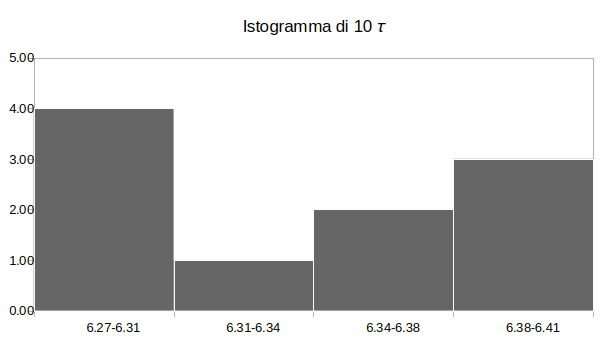
\includegraphics[width=0.8\textwidth]{Immagini/istogramma_dinamico_4.png}
    \captionof{figure}{Istogramma delle 10 misure.}
\end{minipage}

\vspace{0.8cm}

% ==========================================
% MASSA 5
% ==========================================
\subsubsection*{Configurazione Massa $m_5 = 49.99$ g}
\noindent
\begin{minipage}[c]{0.45\textwidth}
\centering
\small
\begin{tabular}{ccc}
\hline
\textbf{Ripetizione} & \textbf{Scarico (s)} & \textbf{Carico (s)} \\ \hline
1  & 4.46 & 7.32 \\
2  & 4.40 & 7.24 \\
3  & 4.47 & 7.32 \\
4  & 4.38 & 7.32 \\
5  & 4.41 & 7.26 \\
6  & 4.40 & 7.29 \\
7  & 4.35 & 7.30 \\
8  & 4.36 & 7.29 \\
9  & 4.37 & 7.27 \\
10 & 4.38 & 7.36 \\ \hline
\end{tabular}
\captionof{table}{Tempi grezzi (5 oscillazioni) per la Massa 5.}
\label{tab:dinamica_massa5}
\end{minipage}
\hfill
\begin{minipage}[r]{0.70\textwidth}
    \centering
    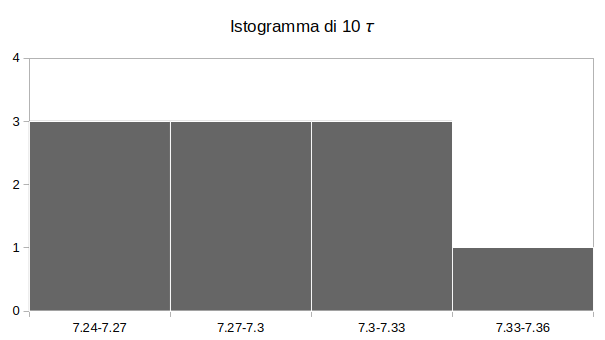
\includegraphics[width=0.8\textwidth]{Immagini/istogramma_dinamico_5.png}
    \captionof{figure}{Istogramma delle 10 misure.}
\end{minipage}
\subsection{Raccolta dati per il decadimento dell'ampiezza}

Il fenomeno di smorzamento generato dalle forze dissipative è stato studiato analizzando l'evoluzione temporale delle ampiezze massime $A_i$ dell'oscillatore. Le misure sono state raccolte a intervalli regolari di $\Delta t = 15\text{ s}$ per una durata complessiva di $90\text{ s}$.

\begin{table}[htbp]
\centering
\caption{Valori sperimentali delle ampiezze massime $A_i$ registrate a intervalli di $15\text{ s}$ e relativi rapporti adimensionali $A_i/A_0$.}
\label{tab:ampiezze}
\begin{tabular}{ccc}
\hline
$t_i$ (s) & $A_i$ (cm) & $A_i/A_0$ \\ \hline
15        & 22.7       & 1.247     \\
30        & 22.2       & 1.220     \\
45        & 21.8       & 1.198     \\
60        & 21.5       & 1.181     \\
75        & 21.2       & 1.165     \\
90        & 20.8       & 1.143     \\ \hline
\end{tabular}
\end{table}


\section{Analisi dati}
\subsection{Stima di k}
\subsubsection{Metodo statico}
\subsubsection*{Dipendenza di $l_i$ da $m_i$}
L'analisi dei dati per il metodo statico ha previsto inizialmente la verifica della seguente
relazione tramite metodo grafico:
$$\Delta l \propto m$$
Come previsto dal modello teorico, infatti:
$$\Delta l = \frac{g}{k} m$$

\begin{figure}[htbp]
    \centering
    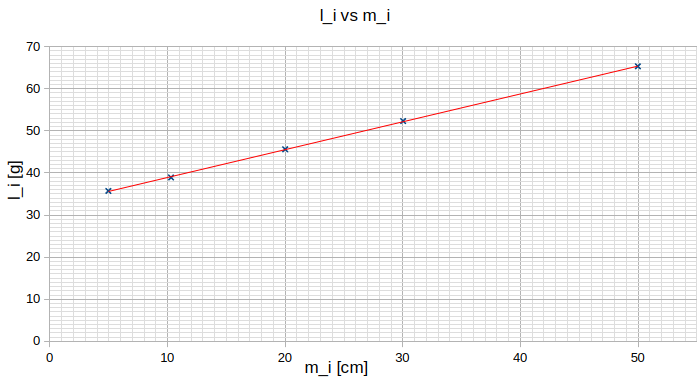
\includegraphics[width=0.8\textwidth]{Immagini/Statico_lvsm.png}
    \caption{Proporzionalità diretta tra $l_i$ e $m_i$}
\end{figure}
Le incertezze associate alle misure di lunghezza e massa sono trascurabili rispetto alla scala
adottata nel grafico e pertanto non sono visibili.

\subsubsection*{Misura di k, metodo statico}
Secondo il modello teorico delineato per il metodo statico, k risulta essere:
$$k_i = \frac{m_ig}{l_i-l_s}$$
con errore:
$$\Delta k_i = k_i(\frac{\Delta m_i}{m_i} + 2\frac{\Delta l}{l_i-l_s})$$

\begin{table}[H]
\centering
\caption{Dati sperimentali raccolti per la determinazione della costante elastica $k$. La lunghezza a riposo della molla è $l_s = 32.4\,\text{cm}$ .}
\label{tab:dati_molla}
\begin{tabular}{cc}
\toprule
$k_i$ (N/m) & $\Delta k_i$ (N/m) \\
\midrule
1.477 & 0.048 \\
1.555 & 0.025 \\
1.486 & 0.012 \\
1.480 & 0.008 \\
1.491 & 0.005 \\
\bottomrule
\end{tabular}
\end{table}

Come stima per $k$ è stato adottato l'ultimo valore, corrispondente all'allungamento massimo.
Infatti, all'aumentare di ($l_i - l_s$), si minimizza l'impatto di tale termine nella propagazione degli errori.

Il medesimo ragionamento si applica alla massa. L'approccio adottato è vincolato dalla mancanza di indipendenza delle misure, in quanto $l_s$ è stata misurata una sola volta all'inizio dell'esperienza.
$$k = (1.491 \pm 0.005)\,\text{N/m}$$
\begin{figure}[H]
    \centering
    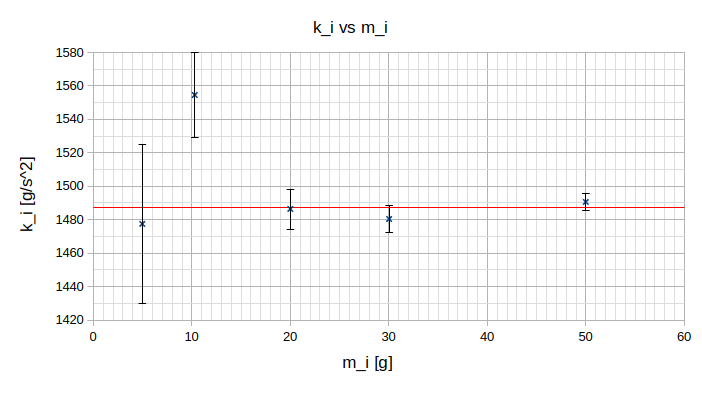
\includegraphics[width=0.8\textwidth]{Immagini/Statico_kvsm.png}
    \caption{Grafico di compatibilità dei $k_i$}
\end{figure}
%%%%fine metodo statico%%%%

\subsubsection{Metodo dinamico}
\subsubsection*{Calcolo senza usare un modello}

Sono stati calcolati i valori dei periodi medi $\bar{T_i}$ per ogni $m_i$ associato con il rispettivo errore $\sigma_{\bar{T_i}}$.
Sono stati valutati anche i valori $\bar{T_{0}}$ corrispondenti ai periodi medi a piattino scarico; ogni set di masse possiede il proprio valore di riferimento al fine di garantire l'indipendenza delle misure.

Il valore di k quindi risulta:
$$k_i = 4\pi^2\frac{m_i}{\overline{T}_i^2 - \overline{T}_{0,i}^2}$$
Con errore associato $\sigma_{k_i}$ ignorando i contributi delle masse:
\begin{equation*}
    \sigma_{k_i} \approx 2 k_i \cdot \frac{\sqrt{\overline{T}_i^2 \sigma_{\overline{T}_i}^2 + \overline{T}_{0,i}^2 \sigma_{\overline{T}_{0,i}}^2}}{\overline{T}_i^2 - \overline{T}_{0,i}^2}
\end{equation*}





\begin{table}[htbp]
    \centering
    \begin{tabular}{cccccccc}
        \hline
        $m_i$ [g] & $\bar{T}_i$ [s] & $T_{0,i}$ [s] & $k_i$ [N/m] & $\sigma_{T_i}$ & $\sigma_{T_0,i}$& $\sigma_{k_i}$ \\
        \hline
        4.97  & 0.9866 & 0.8904 & 1.087 & 0.005 & 0.004 & 0.07\\
        10.30 & 1.0354 & 0.885  & 1.408 & 0.005 & 0.002 & 0.05\\
        20.00 & 1.1708 & 0.8874 & 1.354 & 0.006 & 0.003 & 0.03\\
        30.03 & 1.2672 & 0.8836 & 1.437 & 0.004 & 0.002 & 0.02\\
        49.99 & 1.4594 & 0.8796 & 1.455 & 0.002 & 0.003 & 0.01\\
        \hline
    \end{tabular}
\end{table}

Il valore finale di $k$ è stato calcolato mediante una media pesata sulle incertezze $\sigma_{k_i}$:
$$k = (1.443 \pm 0.007) \text{ N/m}$$

\begin{figure}[H]
    \centering
    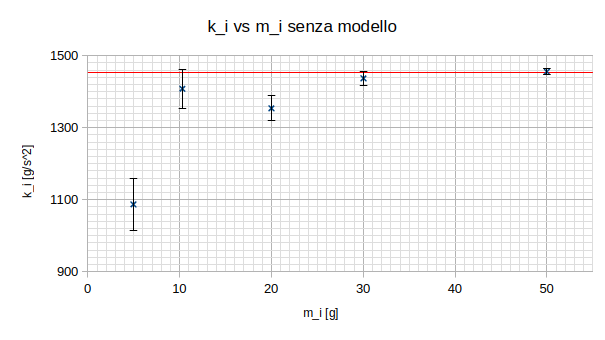
\includegraphics[width=0.8\textwidth]{Immagini/Compatibilita_nmodello_dinamico.png}
    \caption{Grafico di compatibilità dei $k_i$ senza l'utilizzo del modello della massa efficace.}
\end{figure}
\subsubsection*{Calcolo con modello della massa efficace}
Utilizzando gli stessi valori per i periodi del modello precedente è stata calcolata la costante 
utilizzando il modello della massa efficace con la seguente:
$$k_i = 4\pi^2 \frac{M_{tot}}{T_i^2} \quad,\quad  M_{tot} = \frac{m_m}{3}+m_p+m_i$$
Per quanto riguarda il $\sigma_{k_i}$ invece:
$$\sigma_k^2 = k^2\left[\left(\frac{\sigma_{M_{tot}}}{M_{tot}}\right)^2+4\left(\frac{\sigma_{T_i}}{T_i}\right)^2\right]$$
Mentre l'incertezza $\sigma_{M_{tot}}$ è data da:
$$\sigma_{M_{\text{tot}}} = \sqrt{\left(\frac{\sigma_{m_m}}{3}\right)^2 + \sigma_{m_p}^2 + \sigma_{m_i}^2} = \sqrt{\frac{19}{9}} \cdot \sigma_m $$

\begin{table}[htbp]
    \centering
    \begin{tabular}{cccccccc}
        \hline
        $M_{tot}$ [g] & $\bar{T}_i$ [s] & $k_i$ [N/m] & $\sigma_{T_i}$ & $\sigma_{k_i}$ \\
        \hline
        35.07  & 0.9866 & 1.422 & 0.005 & 0.014 \\
        40.40 & 1.0354  & 1.488 & 0.005 & 0.014 \\
        50.10 & 1.1708  & 1.443 & 0.006 & 0.015 \\
        60.13 & 1.2672  & 1.478 & 0.004 & 0.009 \\
        80.09 & 1.4594  & 1.485 & 0.002 & 0.004 \\
        \hline
    \end{tabular}
\end{table}
$k$ è quindi stato calcolato con una media pesata dagli errori $\sigma_{k_i}$:
$$k = (1.478 \pm 0.003) \text{ N/m}$$

\begin{figure}[H]
    \centering
    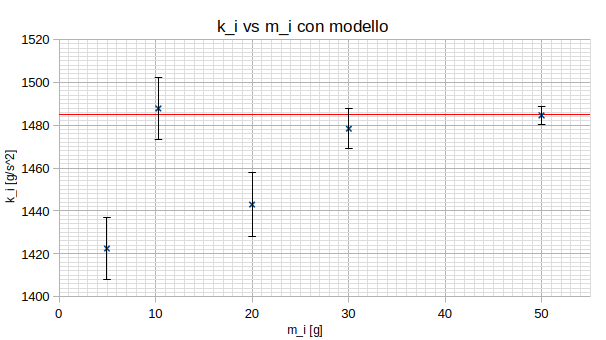
\includegraphics[width=0.8\textwidth]{Immagini/Compatibilita_modello_dinamico.png}
    \caption{Grafico di compatibilità dei $k_i$ con l'utilizzo del modello della massa efficace.}
\end{figure}

\subsection{Stima di $\gamma$}
Per l'analisi del coefficiente di smorzamento $\gamma$ sono stati adottati due approcci:

\begin{enumerate}
    \item \textbf{Verifica puntuale della costanza di $\gamma$ (Analisi delle fluttuazioni):} 
    In prima istanza, l'equazione teorica del decadimento esponenziale $A_i = A_0 e^{-\gamma(t_i-t_0)}$ è stata invertita per calcolare il valore del coefficiente d'attenuazione associato a ogni singolo punto sperimentale:
    \begin{equation*}
        \gamma_i = \frac{1}{t_i - t_0} \ln\left(\frac{A_0}{A_i}\right)
    \end{equation*}
    Ciascun valore $\gamma_i$ è stato corredato del proprio errore sperimentale $\Delta\gamma_i$, stimato mediante la legge di propagazione degli errori massimi:
    \begin{equation*}
        \frac{\Delta\gamma_i}{\gamma_i} = \frac{2\Delta t}{t_i - t_0} + \frac{2\Delta A}{\frac{A_0}{A_i} \ln\left(\frac{A_0}{A_i}\right)}
    \end{equation*}
\begin{figure}[H]
    \centering
    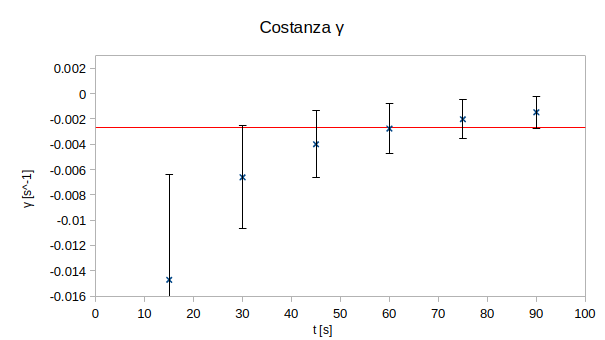
\includegraphics[width=0.8\textwidth]{Immagini/Costanza_gamma.png}
    \caption{Si nota che tutti i valori di $\gamma$ (tranne il primo) sono compatibili con un valore costante}
\end{figure}
    
    \item \textbf{Linearizzazione e Fit Lineare (Stima ottimale del parametro):}
    Una volta accertata la natura costante del parametro, si è proceduto alla stima numerica ottimale di $\gamma$ mediante la tecnica della linearizzazione logaritmica. Definendo le variabili trasformate $Y_i = \ln(A_0/A_i)$ e $X_i = t_i - t_0$, il modello esponenziale assume la forma lineare di una retta passante per l'origine $Y = mX$, dove il coefficiente angolare $m$ coincide esattamente con $\gamma$. 
    
    L'applicazione dell'algoritmo dei minimi quadrati consente di trovare un valore di $m$ con relativo errore:
    \begin{align*}
        m &= 0.001122267\text{ s}^{-1} \\
        \Delta m &= 4.57784 \times 10^{-5}\text{ s}^{-1}
    \end{align*}
\end{enumerate}
\begin{figure}[H]
    \centering
    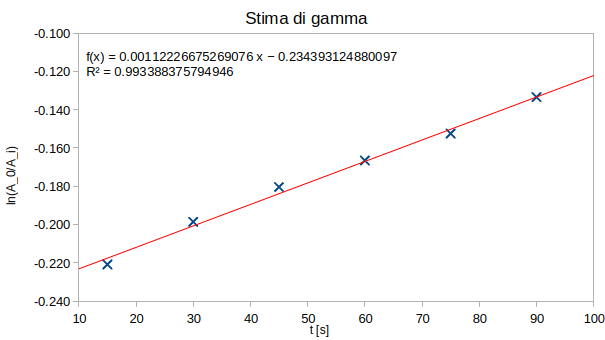
\includegraphics[width=0.8\textwidth]{Immagini/Regressione_lambda.png}
    \caption{Linearizzazione per ricavare $\gamma$ come coefficiente angolare}
\end{figure}

Quindi il valore di $\gamma$ è:
\begin{equation*}
    \gamma = (11.2 \pm 0.5) \times 10^{-4}\text{ s}^{-1}
\end{equation*}

\section{Conclusioni}
In questa esperienza è stata determinata la costante elastica $k$ di una molla elicoidale (valore nominale = 1.5 N/m) confrontando un approccio statico e due varianti di un approccio dinamico. I risultati finali ottenuti sono:
\begin{itemize}
    \item Metodo statico: $k_{\text{stat}} = (1.491 \pm 0.005) \text{ N/m}$
    \item Metodo dinamico (senza modello): $k_{\text{din1}} = (1.443 \pm 0.007) \text{ N/m}$
    \item Metodo dinamico (con massa efficace): $k_{\text{din2}} = (1.478 \pm 0.003) \text{ N/m}$
\end{itemize}


Confrontando la stima statica $k_{\text{stat}}$ e la migliore stima dinamica $k_{\text{din2}}$, si osserva una discrepanza marginale (pari a circa $2\sigma$ combinati). 

Infine, lo studio della dissipazione ha permesso di quantificare il coefficiente di smorzamento, risultato pari a $\gamma = (11.2 \pm 0.5) \times 10^{-4}\text{ s}^{-1}$. Essendo $\gamma \ll \omega_0$ (condizione di smorzamento debole), l'assunzione iniziale di poter trascurare le forze d'attrito per il calcolo del periodo di oscillazione e per la stima di $k$ nel metodo dinamico risulta, a posteriori, rigorosamente giustificata.





\end{document}